Consider an application with six tasks, denoted ``T0''--``T5'', and a heterogeneous architecture with two cores, labeled ``PE0'' and ``PE1''. The task graph of the application is given in \figref{fig:task-graph} along with the execution times for both cores. The period of the application is 0.06 seconds. A first alternative mapping and schedule, and the resulting SSDTP are shown at the top of \figref{fig:motivation} (where the hight of a task represents its relative dynamic power consumption). It can be observed that initially PE0 is experiencing three thermal cycles. If we change the mapping of T5 and move it to PE1, we achieve two thermal cycles of PE0 instead of three. Finally, if we vary the schedule as well and change the order of T1 and T3, the number of cycles of PE0 becomes one. Using the reliability model from \secref{sec:reliability-model}, we observe improvements in the lifetime of 44.69\% and 54.53\%, respectively, relative to the initial configuration.
\begin{figure}
  \centering
  \subfloat[The task graph.]{
    \label{fig:task-graph}
    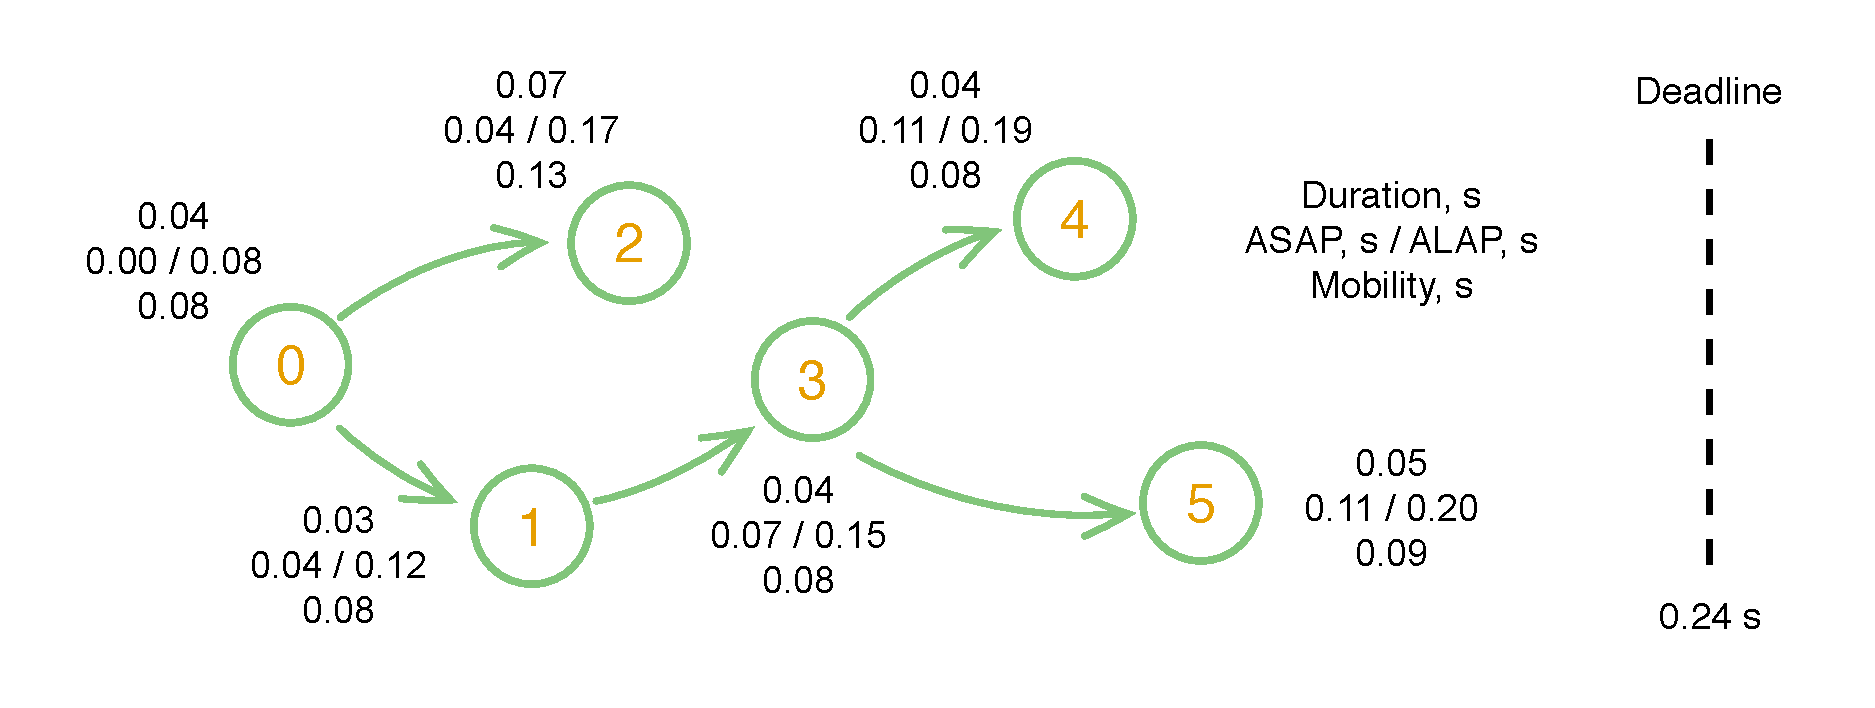
\includegraphics[width=0.8\linewidth]{assets/task-graph.pdf}
  }
  \vspace{-10pt}

  \subfloat[Alternative mappings and schedules.]{
    \label{fig:motivation}
    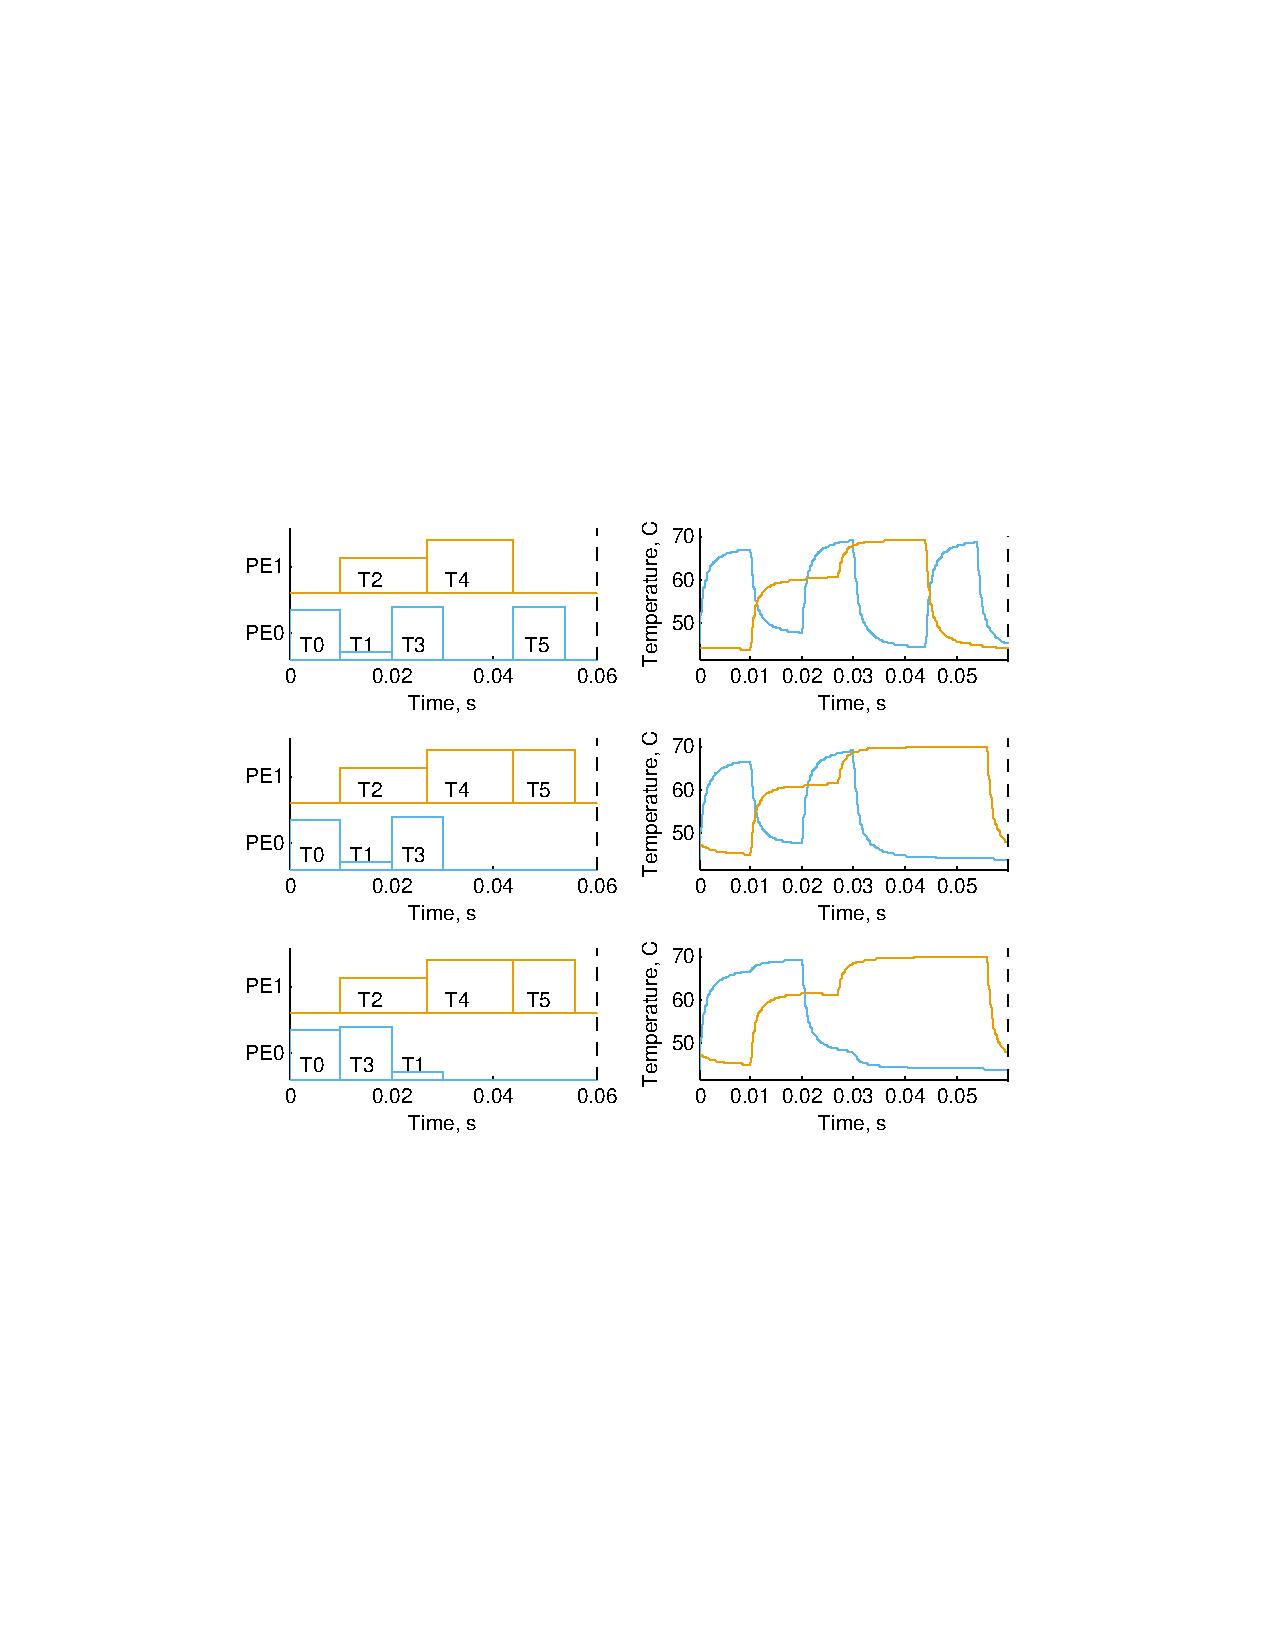
\includegraphics[clip=true, trim=30 30 30 10, width=0.8\linewidth]{assets/motivation.pdf}
  }
  \caption{Motivational example.}
  \vspace{10pt}
\end{figure}
